% #####################################################
% #####################################################
% #####################################################
\setchapterimage[4cm]{figures/chap5/ITER_Robots2018} % Optionally specify theheight
\setchapterpreamble[u]{\margintoc}
\chapter{Fusion Education}\label{chap:Fusion Education}

\epigraph{What one fool could understand, another can.}{R.P.~Feynman}

% ################################################################
% ################################################################
% ###############################################################
\section{ITER Robots}
\marginnote{Parts of this section have been taken from \citeauthyear{martins2020}}

The ITER Robots competition is organized for school children located in Provence-Alpes-Côte d’Azur in order to introduce the various challenges ITER is facing. This contest aims to bring technical challenges to students into a cross-disciplinary approach.
\begin{marginfigure}
	\centering
	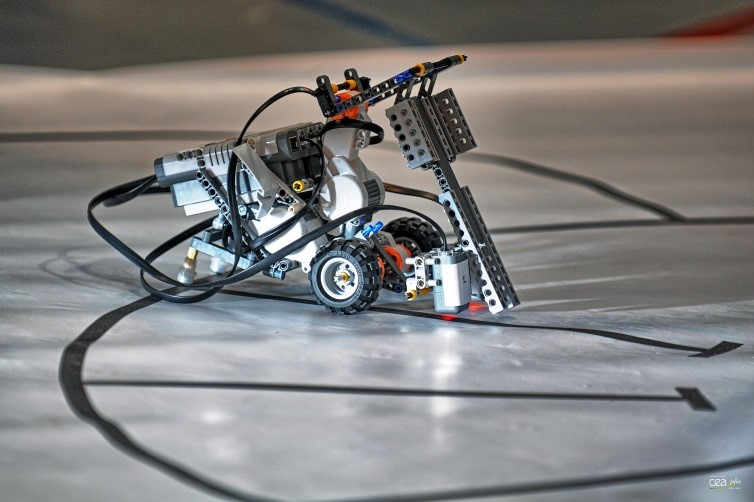
\includegraphics[width=1.0\linewidth]{figures/chap5/ITER_Robots_1}
	\caption{Picture of a robot LEGO MINDSTORMS® based during the TRANSPORT challenge. (©C.Roux, CEA)}
	\label{fig:iterrobots1}
\end{marginfigure}
The challenge is to build a reduced scale robot to simulate a maintenance situation inside the future ITER Tokamak machine, namely the remote handling of components in a hostile environment. The robots' architecture was initially based on LEGO bricks with sensors controlled by a LEGO MINDSTORMS® programmable unit (Figure~\ref{fig:iterrobots1}). When considering kids and school capabilites, others technologies  have been introduced after such as Arduino® (or equivalent) boards and 3D printed elements. Each robot is named by its creators. The purpose of the contest is to challenge team composed of full classes or few students from primary schools (aged from 10 to 11), middle schools ("collège", aged from 11 to 15) and high schools ("lycée", aged from 16 to 18) to remote handling problematics. Junior high school team of students can be held within their established technological school programmes (in 7th, 8th and 9th grades or within interdisciplinary educational programme projects). Secondary school students can integrate the competition to their first and final year of high school technological programmes (in science, engineering or technology). In 2019, ITER Robots becomes part of the regular syllabus for primary school students as a technology lesson.

\begin{marginfigure}
	\centering
	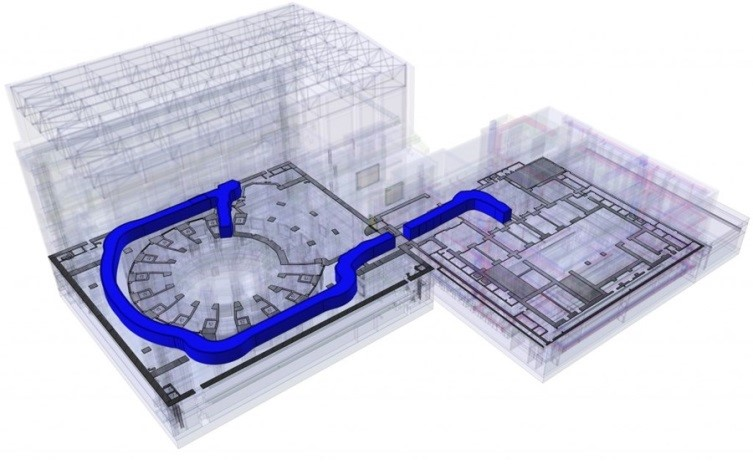
\includegraphics[width=1.0\linewidth]{figures/chap5/ITER_Robots_2}
	\caption{Due to the limited space in the nuclear environment of ITER, transport cask trajectories are complex. In blue: sample trajectory between a port in Tokamak Building (left) and the hot cell facility (right). (©iter.org)}
	\label{fig:iterrobots2}
\end{marginfigure}

Scaled-down and adapted challenges involving totally autonomous robots illustrate the real-life problems ITER will be facing. The challenges are downscaled replications of real remote handling tasks that will occur in the future facility. Indeed, when the nuclear phase of the experiment will begin, some areas of the tokamak become man access restricted. Inspections or repair of any of the tokamak components (weighing up to 50 tonnes) in the restricted areas will thus require reliable and robust remote handling techniques. In brief, the overall maintenance strategy of the tokamak consists on transporting the large components from their locations in the reactor to the repair workshops (called hot cells) for technical operations (cleaning, replacement of components, etc.), see Figure~\ref{fig:iterrobots2}.

Like the ITER scientists, students are actively involved for a period of 4 to 6 months in project management, such as project analysis, planning and testing. Students must combine the theoretical concepts learned at school and apply lessons during robots design, programming and testing activities. 

\begin{marginfigure}
	\centering
	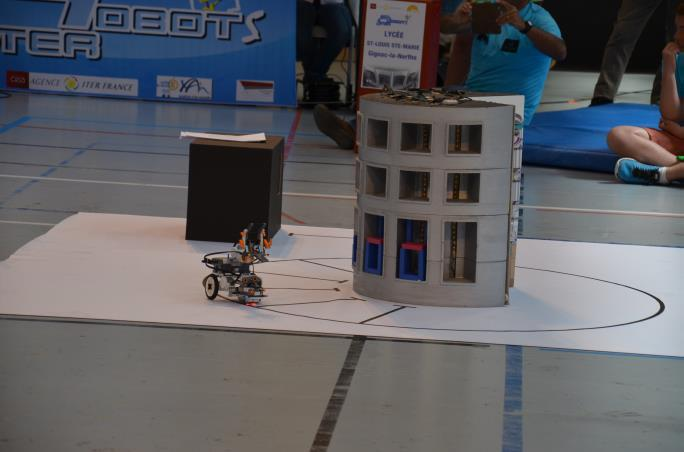
\includegraphics[width=1.0\linewidth]{figures/chap5/ITER_Robots_3}
	\caption{Picture of the \textit{TRANSPORT} challenge. The robot must autonomously follow the tracks plotted on the floor and pick a brick (here in red) in each "port" of the ITER mock-up (in the middle). Once got, the robot must bring back the brick to the "hot-cell" (black zone at the left of the figure).}
	\label{fig:iterrobots3}
\end{marginfigure}

Technical issues are not the only challenges that ITER scientists must face. Working in a multicultural environment, with worldwide working cultures and lifestyles is also an important aspect of the programme. Thus, in addition to the robotics challenge, the competition includes a broad general knowledge preparation about the ITER project itself and its seven members (culture, geography, history, economy, etc.). Humanities teachers from nearby middle schools are involved in the competition and teams are evaluated through a quiz during the day of the finals. Also, to enforce the communication side, teams shall prepare a dedicated booth and magazine illustrating their work along the year. A dedicated jury evaluates the work the day of the contest.


The number of participants in the ITER Robots competition, created by the Agence ITER France in 2012, is growing, with more than 600 participants from 30 regional education establishments in the 2019 edition. As part of their technical and science curriculum, students work in teams, for over 6 months, to acquire technical skills and knowledge on robotics and fusion energy, solve problems, develop communication skills, and run their projects. Teachers enjoy the practical approach developed with the ITER Robots competition. This contest corresponds to the current educational “cross disciplinary approach”, from technology to French, foreign languages as well as history, from science to general international knowledge. Disappointments are also part of the adventure and the intermediate project reviews are a good opportunity to boost students and to give them precious tips. The contest day, each team's robot undertakes a number of tasks evaluated by jury composed of ITER and CEA engineers. Teams are also evaluated on communication skills and fusion energy knowledge. 


\marginnote{\href{https://www.youtube.com/watch?v=z6rhHYrs980}{ITER Robots 2018 teaser video}}

Robotics provides a fun and exciting environment for school students and is an ideal subject to get them interested to science, technology, engineering, and math (STEM). ITER is a unique mega-project, which is currently challenging all present technological domains (cryogenics, superconducting, vacuum, high temperature plasma, etc.). Combined together, ITER Robots is a challenge introducing collegiality, experimentation and project management to the students in order to solve a real problem, mimicking an important aspect of ITER. During the challenge, students can benefit from a scientific environment by being in contact with scientists, engineers and technicians. This opportunity has proved to encourage some of them to be interested in engineering or science careers. This is particularly important, especially from students coming from disadvantaged areas, as they never envisaged it possible to work on such fields. This is also important to limit young people's disaffection for scientific and technical careers. 


% ################################################################
% ################################################################
% ################################################################
\section{Master Fusion}
\marginnote{Parts of this section comes from the paper \citeauthyear{hillairet2020}. The author would like to thanks Joëlle Achard, without whom this work would not have been possible. The author would like to thanks the organizers of the Cadarache IRFM master fusion events: Remy Guirlet, Nicolas Fedorzak, Pascale Monier-Garbet, Rémi Douvenot from ENAC/Toulouse, current and former members and PhD students of the IRFM RF group for their various supports in these activities and of course the students themselves. }

In order to train the future fusion scientists and engineers, French and European master programs exist to provide teaching on plasmas sciences and associated technologies. These master's programs deal with most scientific and technological fields related to the ionized media via theory, numerical modelling, material sciences, cryotechnology and superconductivity and instrumentation in extreme environments. However, for a vast majority of them, no dedicated courses are provided on RF sciences and technologies, despite their large use on fusion research facilities. 

During two weeks at the beginning of the civil year, both French and European master students gather in the Cadarache research centre in order to participate in small groups to hands-on organized by fusion researchers. The topics of these hands cover the large spectrum of fields used in fusion research: cryotechnology and superconductors, infra-red measurements, numerical modelling, tokamak data analysis, virtual reality, etc. 

Among these hands-on, some are devoted to RF component measurements and analysis and are described in more details in \sidecite{hillairet2020}. Specific hands-on have been devoted to ICRF and LHCD antenna component RF measurements: the high voltage probe calibration, the electrical scheme of possible ICRH antenna, the measurements of a mode converter or a multijunction RF performances. This Section only describes the later two hands-on dedicated on WEST LHCD antenna components. 

% ########################################################
% ########################################################
\subsection{LHRF hands-on}

\begin{marginfigure}
	\centering
	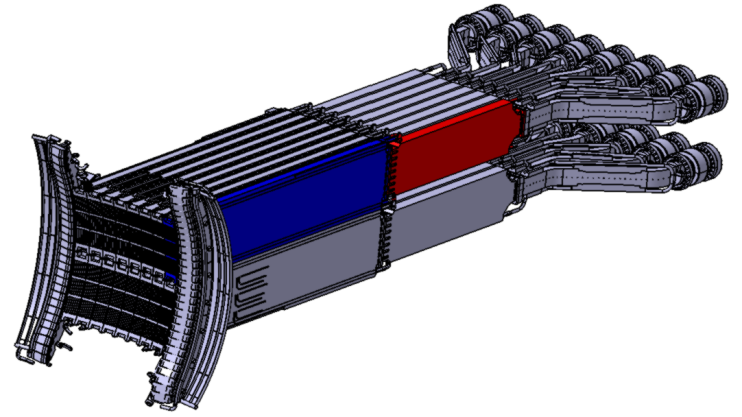
\includegraphics[width=1.0\linewidth]{figures/chap5/handson_LH_1}
	\caption{CAD view of a WEST Lower Hybrid antenna (aka "LH1"). The red part is the $\TE_{10}$-$\TE_{30}$ Mode Converter. The Blue part is the "multijunction". Dimensions: 0.7x0.7x5~m. Weight: a few tons. }
	\label{fig:handsonlh1}
\end{marginfigure}

Two hands-on have been proposed to the students on two RF components constituting the real WEST LH launchers: a mode converter (in red in Figure~\ref{fig:handsonlh1}) and a "multijunction" (in blue in Figure~\ref{fig:handsonlh1}). These RF components have multiple functions detailed in Section~\ref{{sec:LHCD_antennas_general}}, but the main one is to split the RF power coming from the klystron to numerous waveguides facing the plasma. 

\subsubsection{$\TE_{10}$-$\TE_{30}$ mode converter}

During this hands-on, students measure the RF performances of a $\TE_{10}$-$\TE_{30}$ mode converter prototype (Figure 4) which has been developed for the LH1 antenna \sidecite[+1cm]{bibet2000}. The performances of an RF device being generally expressed via scattering parameters (or S-parameters), a general introduction to the S-parameter is given to the student groups in the first hours of the hands-on. 

\begin{marginfigure}
	\centering
	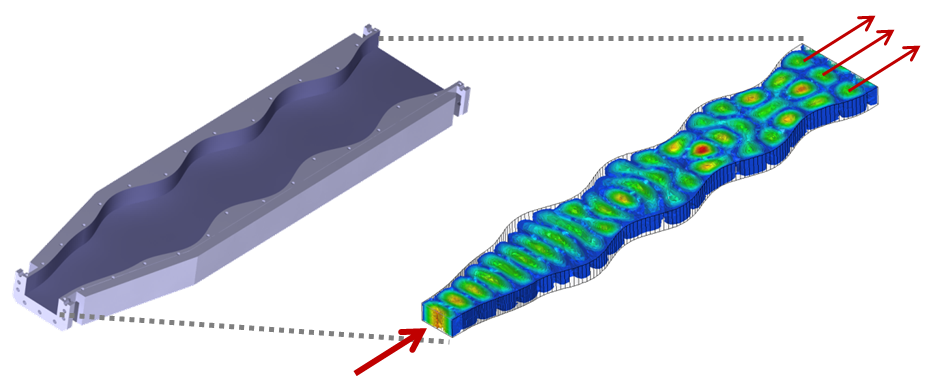
\includegraphics[width=1.0\linewidth]{figures/chap5/handson_LH_2}
	\caption{CAD Internal view and its associated RF modelling (electric field).}
	\label{fig:handsonlh2}
\end{marginfigure}

Like a role-playing game, the advisors ask the students to act as an RF technician who have been asked by his/her head to characterize this $\TE_{10}$-$\TE_{30}$ mode converter prototype and to report its performances as soon as possible. Unfortunately, the prototype had not been built exactly as designed: during the brazing operation which has been performed to assemble all the stainless-steel and copper parts of the structure, the mechanical pressure was not homogeneous, leading to less than a millimetre local deformations. This is however sufficient to perturb the RF performances: the mode converter and its splitter is found to not split evenly the power in three (-4.77~dB) but instead to -5.4, -4.2 and -5.3~dB for the left, central and right branches respectively at the frequency of interest (3.7~GHz). 

\begin{figure*}
	\centering
	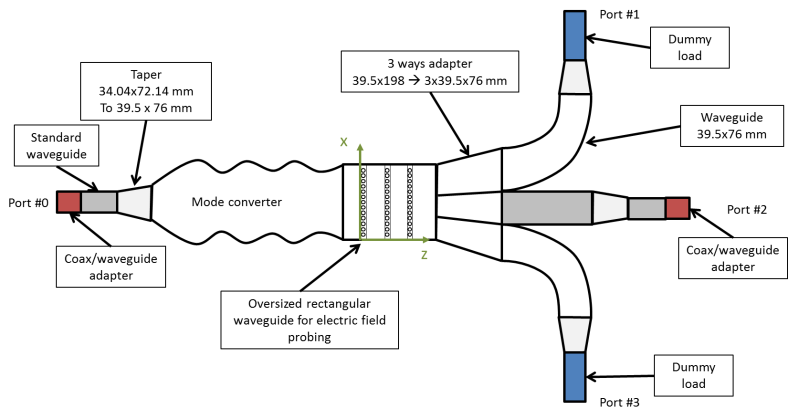
\includegraphics[width=0.55\linewidth]{figures/chap5/handson_LH_3}
	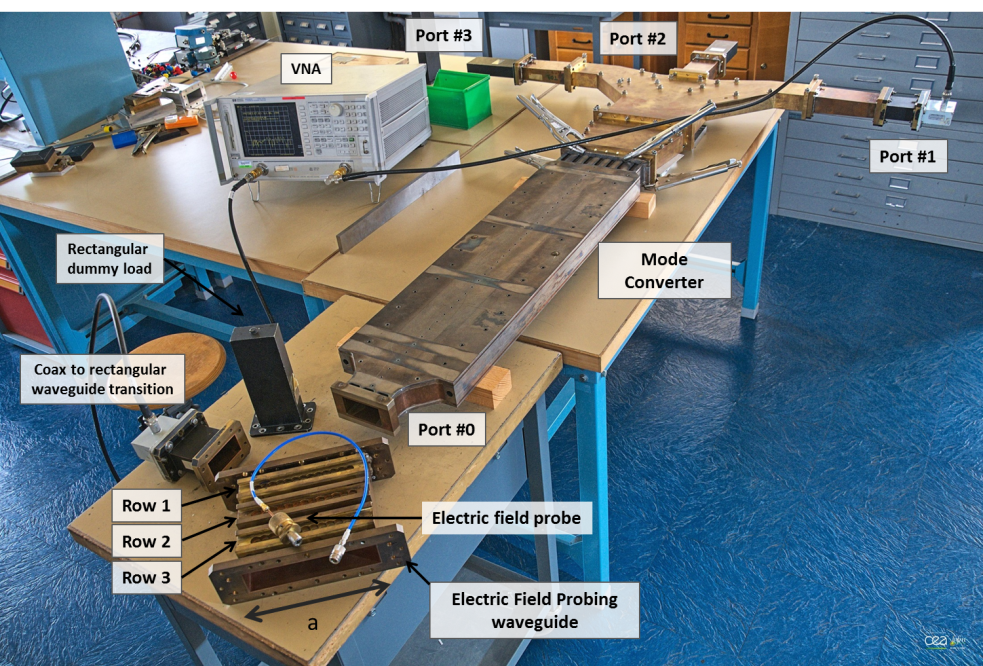
\includegraphics[width=0.44\linewidth]{figures/chap5/handson_LH_4}
	\caption{Left: Illustration of the measurement setup. Right: Picture of the mode converter setup.}
	\label{fig:handsonlh3}
\end{figure*}


However, the students are not told of this fact (which retrospectively was discovered once the RF measurements had been made during prototype acceptance test). They thus find unexpected results and the supervisors act as if they were surprised, telling the students that the "RF design" is supposed to be perfect. Generally puzzled by their finding, very few students guess at first that a problem may have occurred during manufacturing. Students are thus asked how sure of their measurements they are, which is a good opportunity to discuss and explain the importance of calibrations, power conservation, statistics and uncertainties in experimental physics.

In order to help them to find the origin of the mode converter problem, students are provided the opportunity to measure the electric field at the end of the mode converter, in the $\TE_{30}$ section (output), using a dedicated waveguide pierced by an array of very small holes inserted between the mode converter and the 3-ways adapter and an appropriate probe collecting a fraction of the electric field propagating inside the waveguide (Figure~\ref{fig:handsonlh2}). Once measured in various positions (Figure~\ref{fig:handsonlh3}), students are asked from these data to deduce the mode content inside the mode converter, i.e. the amplitude of the modes propagating inside the structure to complete their analysis. This task requires the students to make a numerical model of the electric field inside the waveguide, as a combination of TE modes. Since 2011, this problem had been solved using various approaches and computer languages by the students: from least-squares fits to Fourier transforms, with Matlab, Python, Excel or even compiled languages such as Fortran or C. 


\begin{figure*}
	\centering
	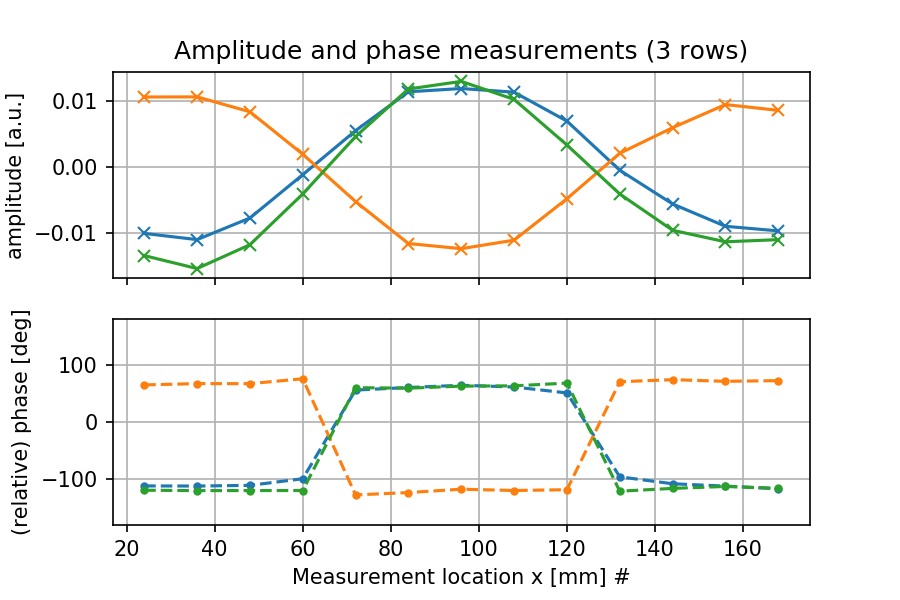
\includegraphics[width=0.49\linewidth]{figures/chap5/handson_LH_5}
	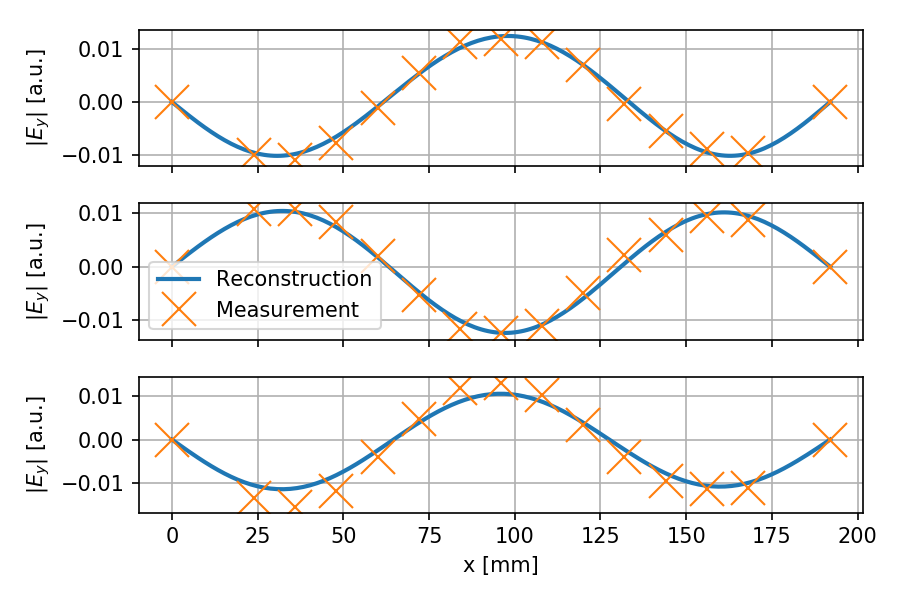
\includegraphics[width=0.49\linewidth]{figures/chap5/handson_LH_6}
	\caption{Left: Measurement of amplitude and phase at various positions in the TE30 section of the TE10-TE30 mode converter for the three rows. Right: Once the unknown TE mode coefficients have been found, one can reconstruct the electric field everywhere in the waveguide section and compare to the measurements. In this example, additional points have been added at the edges of the waveguide, where the electric field is zero, to additionally constrain the model.}
	\label{fig:handsonlh5}
\end{figure*}


\subsubsection{LHCD Multijunction Antenna Prototype}

\begin{marginfigure}
	\centering
	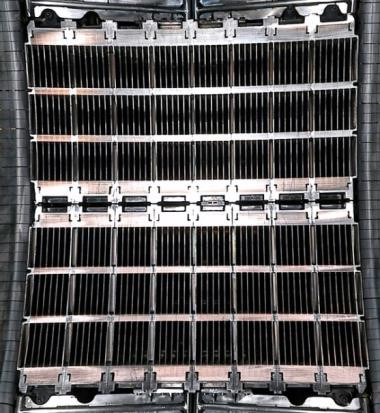
\includegraphics[width=0.8\linewidth]{figures/chap5/handson_LH_MJ_1.png}
	\caption{picture of the WEST LH1 multijunction antenna front face.}
	\label{fig:handsonlhmj1}
\end{marginfigure}

During this hands-on, students have to measure the RF characteristics of a real multijunction mock-up, which was used to validate the LH1 antenna design \cite{bibet2000}. First, they have to understand how a multijunction structure achieves to both split and phase shift the RF power. They have to determine analytically and numerically the spectral power density spectrum excited by the antenna. This quantity is an important parameter for the antenna operation and it corresponds to the spatial Fourier transform of the power density at the antenna mouth (Figure~\ref{fig:handsonlhmj3}).

This first part is thus the opportunity to discuss and clarify how waves can be described either in spatial and spectral domains. The differences between Fourier transform and Discrete Fourier Transforms are also always discussed, since the latter is used in a Fast Fourier Transform algorithm but not always to the awareness of the students. The direction at which the RF waves should be preferentially launched inside the tokamak plasma, which is related to the usual phased array angle, is also discussed.

\begin{marginfigure}
	\centering
	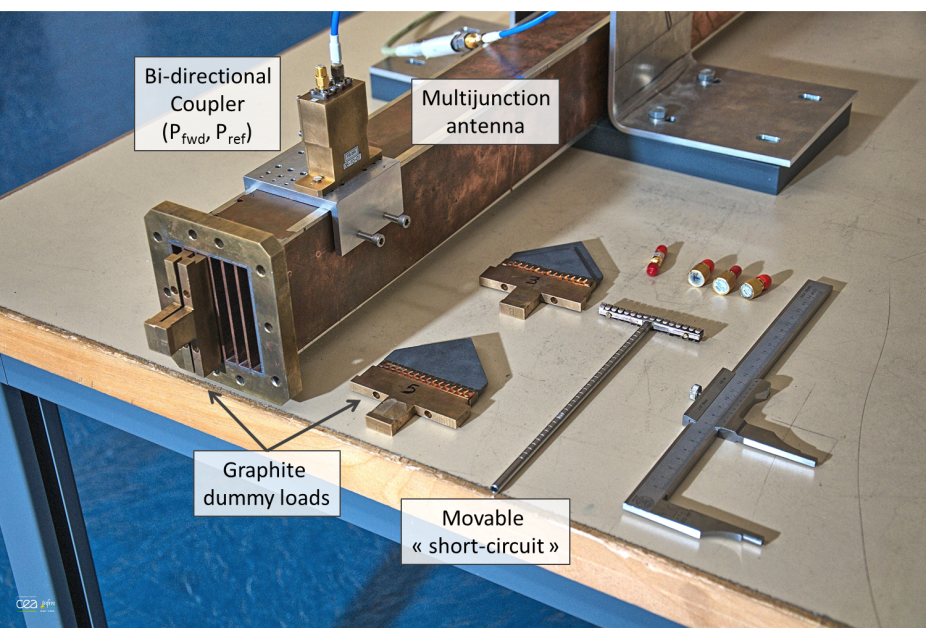
\includegraphics[width=1.0\linewidth]{figures/chap5/handson_LH_MJ_2.png.jpg}
	\caption{Multijunction hands-on setup and description of its components}
	\label{fig:handsonlhmj2}
\end{marginfigure}

Then students can perform RF measurements of the prototype multijunction module. However, since this structure uses thin rectangular waveguides (70x8mm), no standard RF components exist for this task. Specific home-made RF loads and couplers have been built to measure a fraction of the power in each waveguide. Students are then guided to the calibration methods required for these probes, using again specific home-made tools such as tapers, reduced size waveguides and matching loads made in graphite (Figure~\ref{fig:handsonlhmj2}).

Once the prototype measurements have been made, the students can compare their results to their antenna model and discuss the importance of measurement uncertainties and the origin of these uncertainties. Finally, the supervisors give the student a movable short-circuit (Figure~\ref{fig:handsonlhmj2}) which can be inserted inside a reduced waveguide. This short is a rough way to model an arc happening inside the waveguide. Students are then asked if it is possible to (i) detect arcs in the multijunction from the analysis of the reflected power and (ii) if it is possible to locate the arcs in the multijunction? They are then left free to do any measurements they wish to give first insights to these questions. During this part are discussed with them the importance of establishing a proper test protocol (What to do? How to it?) and the expected measured values (too much or not enough data?) to analyse an experimental problem.


\begin{figure*}
	\centering
	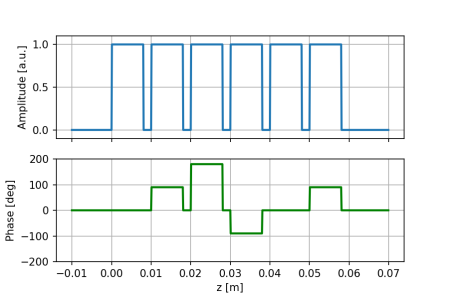
\includegraphics[width=0.49\linewidth]{figures/chap5/handson_LH_MJ_3}
	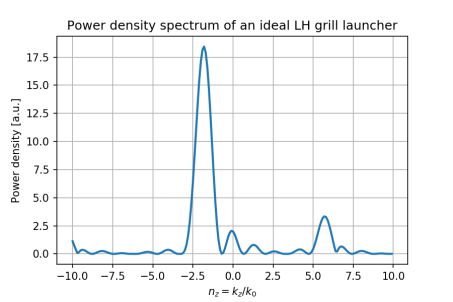
\includegraphics[width=0.49\linewidth]{figures/chap5/handson_LH_MJ_4}
	\caption{Left: Ideal amplitude and phase excitation of the multijunction waveguides. Right: associated power density spectrum}
	\label{fig:handsonlhmj3}
\end{figure*}

\subsection{Summary of this Section}
Over the 8 years since we’ve started the RF hands-on, as part of the IRFM master fusion event, we have been pleased to make students discover the tools and subjects related to plasma RF heating and current drive. As none of the students had followed any RF courses during their scholarship, RF theory and measurements are not definitely easy to them. The challenges were thus to create hands-on for which they can perform RF measurements and data analysis, without having to know the typical knowledge of RF engineering. If the RF hand-on topics are not always their first choices, students are still happy to learn new things, in particular that from design to application, many steps pave the road of researchers and that none of them must be neglected. 

% ###############################################################
% ###############################################################
% ###############################################################
%\section{Com grand public}

% ###############################################################
% ###############################################################
% ###############################################################
%\section{Dim tokamak?}

\clearpage
% ###############################################################
% ###############################################################
% ###############################################################
\section[Open Source Software]{Open Source Software Development}
\marginnote{Parts of this Section are taken from paper \citeauthyear{hillairet2019-1}. The author would like to Alex Arsenovic (and \href{https://github.com/scikit-rf/scikit-rf/graphs/contributors}{the scikit-rf developers}) for the scikit-rf package. 
	
	Since 2019, the author is officially a maintainer of this package.}

Modern science is founded on hypothesis testing and statistical significances of its derived results. Reproducing experiments, experimental or numerical, is the reason why scientists can gain confidence in their conclusions. However, during the last decades, the number of codes and libraries developed at an individual or a laboratory scale only increased. When these tools are not open-sourced, it leads to an obvious reproducibility problem as one should only rely on authors claims. To conform to the necessity of reproducibility in science,  software sources used in physical and engineering researches should ideally be made open when possible \sidecite{ince2012}. The case of RF network manipulation and analysis is no different.  

\href{http://www.scikit-rf.org}{\texttt{scikit-rf}} is a Python package produced for RF/Microwave engineering  \sidecite{arsenovic2018}. The package is licensed under the Berkeley Software Distribution (BSD) licence and is actively developed by volunteers on GitHub. The package provides a modern, object-oriented library for RF network analysis and calibration. Besides offering standard microwave network operations, such as reading/writing Touchstone files (\texttt{.sNp}), connecting or de-embedding N-port networks, frequency/port slicing, concatenation or interpolations, it is also capable of advanced operations such as Vector Network Analyzer (VNA) calibrations, time-gating, interpolating between an individual set of networks, deriving network statistical properties and supports Virtual Instrument for direct communication to VNAs. The package also allows straightforward plotting of rectangular plots (dB, mag, phase, group delay, etc), Smith Charts or automated uncertainty bounds. 

As the package is developed in Python, it makes it naturally compatible with the rich and modern scientific Python libraries \sidecite[-1cm]{millman2011}, for example  \texttt{scikit-learn} for machine learning tasks \sidecite[-0.5cm]{pedregosa2011} or \texttt{PlasmaPy} \sidecite{plasmapycommunity2019} for plasma physics. Using Jupyter notebooks documents\sidecite{kluyver2016}, modelling approaches and results can be shared and even directly reproduced using tools such as \href{https://mybinder.org/}{Binder} or \href{https://colab.research.google.com/}{Google Colab}, by other researchers (or future self) few months or years after work had been made. It also makes it naturally compatible with the rich and modern testing and code coverage frameworks and reproducible modelling approaches using online
virtualization services. Being open-source, using scikit-rf to create the antenna numerical model with reproducible work-flow adds confidence
in the fact that future users could use/maintain and extend it.

At the time of the writing of this manuscript (April 2020), the \texttt{scikit-rf} package has been download more then 50000 times since January 2017 using the Anaconda Python package manager (but this include multiple downloads/user). The number of download of the package on github is of the order of 20 to 50 per 15 days. The mailing list has 124 registered users.